\documentclass{article}

\usepackage{xcolor}
\pagecolor{white}
\usepackage[utf8]{inputenc}
\usepackage{amsmath}
\usepackage{graphicx}
\usepackage{gensymb}
\usepackage{fancyhdr}
\usepackage{lipsum}
\usepackage[margin=0.5in,includefoot]{geometry}
\usepackage{fancyhdr}
\usepackage[normalem]{ulem}
\usepackage{cancel}
\usepackage{amsfonts}
\usepackage{amssymb}
\usepackage{amsbsy}
\usepackage{amsmath}
\usepackage{mathtools}
\usepackage{setspace}

\begin{document}
\section*{Unit 3B Test: Zeros of a Quadratic (2022)}
Grading:\\
knowledge and understanding: ?\\
application: ?\\
thinking: ?\\
communication: 4 + 2 (form)\\

\vskip 1cm

\noindent{(1) Solve the equation $2(x-1)^2-8=0$ [A][3].}
\vskip 0.5cm
\textbf{\color{red}{We}} First move $8$ to the other side of the equation
\[
	2(x-1)^2=8
\]
\[
	(x-1)^2=4
\]
\[
	x-1=\pm2
\]
And therefore $x=1\pm2=3,-1$.
\vskip 1cm
\noindent{(2) Determine the equations of the parabola in vertex form for the following}\\

a.) If the vertex of a parabola is $(3,-5)$ and the y-intercept is at $y=8$ [T][3].
\vskip 0.5cm
\textbf{\color{red}{Since}} the vertex is at $V(3,-5)$, we get the equation is sofar
\[
y=a(x-3)^2-5
\]
Then, since we are given that the y-intercept is at $y=8$, we get the point $(0,8)$, which we will plug in to solve for $a$
\[
	8=a(0-3)^2-5
\]
\[
	a=\frac{13}{9}
\]
Therefore, the final equation is $y=\frac{13}{9}(x-3)^2-5$.
\vskip 1cm
b.) If the parabola $y=x^2$ is stretched by a factor of 5, moved 6 units to the right, and moved 7 units down [T][2]. 
\vskip 0.5cm
hte equation is simply $y=5(x-6)^2-7$, where we have that $5$ because it is stretched by 5, we have $x-6$ for shifting 6 units to the right, and at last we have that $-7$ because it is shifted down 7 units. 
\vskip 1cm
\noindent{(3) Rewrite the equation $y=2x^2+8x+3$ in vertex form and also sketch it [A][3].}
\vskip 0.5cm
\textbf{\color{red}{We}} first factor out a 2 from the first two terms to get 
\[
	y=2(x^2+4x)+3
\]
Then, we see that $(\frac{b}{2})^2=(\frac{4}{2})^2=4$ so we add on $4-4$ inside the parantheses
\[
	y=2(x^2+4x+4-4)+3
\]
Then, we see that $x^2+4x+4=(x+2)^2$ and so we get 
\[
	y=2[(x+4)^2-4]+3
\]
Then, we use the distributive property to distribute the 2 to get 
\[
	y=2(x+4)^2+2(-4)+3=2(x+4)^2-5
\]
And so that is our final equation in vertex form.
\vskip 1cm
\noindent{(4) Sketch the parabola $y=2(x+3)^2-2$. The sketch must include the x-intercept(s), y-intercept, and vertex of the parabola [A][3].}
\vskip 0.5cm
\textbf{\color{red}{From}} this, we see that the vertex is at $(-3,-2)$. Additionally, we plug in $x=0$ to get that the y-intercept is at $y=2(0+3)^2-2=16$. Then, for the x-intercepts, we set $y=0$ to get 
\[
	0=2(x+3)^2-2
\]
\[
	(x+3)^2=1
\]
\[
	x=-3\pm1
\]
And so the x-intercepts are at $(-2,0)$ and $(-4,0)$. Therefore, if you graph it, you will get something like this
\begin{center}
	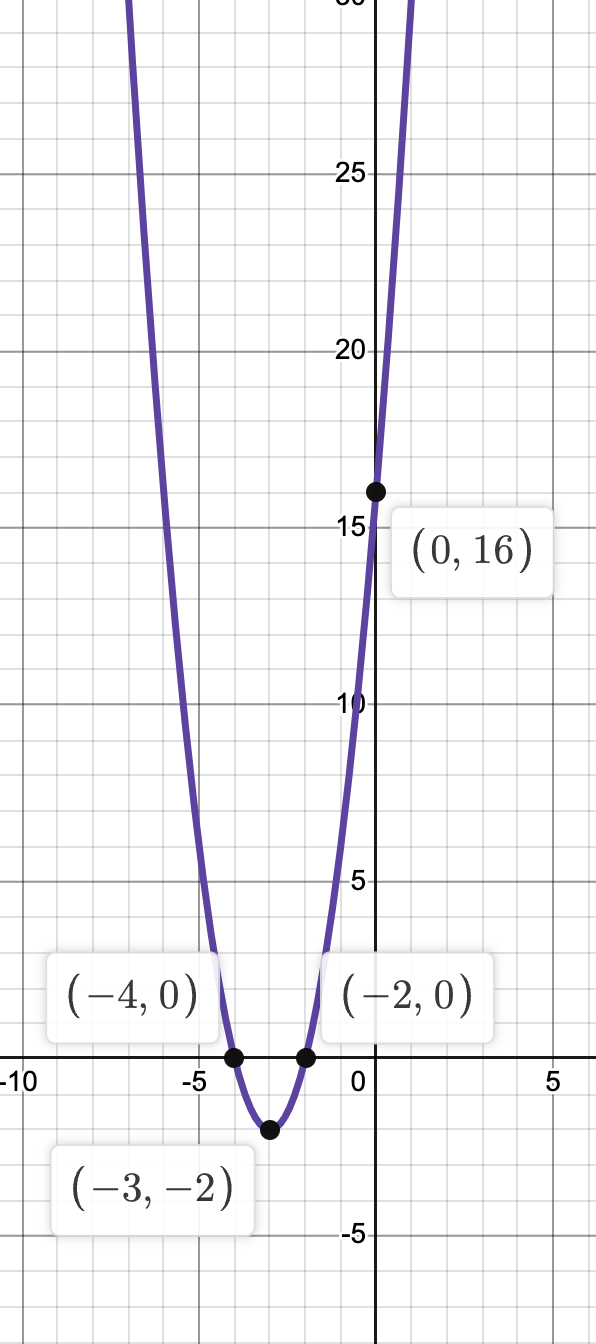
\includegraphics[scale=0.4]{figure8.png}
\end{center}
\vskip 1cm
\noindent{(5) For the parabola $y=3(x-5)^2-6$}\\

a.) Identify the equation for the axis of symmetry, the max/min, and the vertex [K/U][3].
\vskip 0.5cm
\textbf{\color{red}{The}} axis of symmetry is at $x=5$, the minimum is at $y=-6$, and the vertex is at $(5,-6)$.
\vskip 1cm
b.) Describe the transformation of the parabola [C][4].
\vskip 0.5cm
\textbf{\color{red}{Vertically}} stretch by 3, shift 5 units to the right, and shift 6 units down. 
\vskip 1cm
c.) Determine the x-intercept of the parabola [K/U][2].
\vskip 0.5cm 
\textbf{\color{red}{We}} plug in $y=0$ to solve for $x$ and we get 
\[
	3(x-5)^2-6=0
\]
\[
	(x-5)^2=2
\]
\[
	x-5=\pm2
\]
And so therefore the x-intercepts are at $(5+\sqrt{2})$ and $(5-\sqrt{2},0)$.

\end{document}
